
\chapter{Aufbau und Analyse der ETL Prozesse}

\section{Überblick der verwendeten Datenquellen}

\subsection{Numerische Wettervorhersagen}

Heutige Wettervorhersagen basieren auf den aufwendig berechneten
Ergebnissen numerischer Wettermodelle. Diese Modelle versuchen den
Zustand der Atmosphäre und deren Veränderung im Laufe der Zeit als
mathematisches Problem zu beschreiben. Dabei werden die physikalischen
Größen und Beziehungen, die den Zustand und die Veränderung der
Atmosphäre beschreiben, als System partieller Differentialgleichungen
modelliert. Allen Modellen liegen dabei dieselben physikalischen
Gesetzmäßigkeiten, wie die Erhaltungssätze von Energie, Impuls und
Masse, zugrunde, unterscheiden sich aber in der konkreten
mathematischen Formulierung und der numerischen Lösung dieser
Gleichungssysteme.

Um die reale Atmosphäre auf ein Modell abbilden zu können wird eine
Diskretisierung von Raum und Zeit vorgenommen. Dabei wird die
Oberfläche der Erde mit einem aus Dreiecken oder Vierecken bestehenden
Gitternetz überzogen, und die Atmosphäre horizontal in mehrere
Luftschichten aufgeteilt. In Abbildung \ref{gitternetz} ist das
Gitternetz des vom Deutschen Wetterdienst und Max-Planck-Institut für
Meteorologie entwickelten Wettermodells \textit{ICON}
\nomenclature{ICON}{ICOsahedral Non-hydrostatic General Circulation
  Model} zu sehen.

\begin{figure}[h]
  \begin{center}
    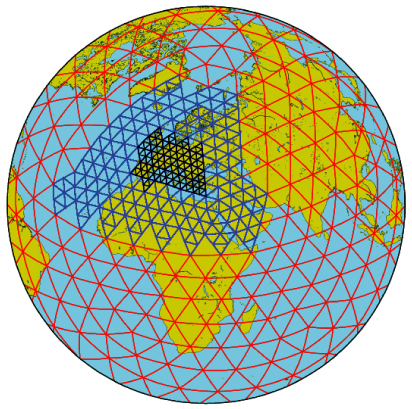
\includegraphics[height=200px]{bilder/gitternetz}
    \caption{Dreiecksgitter des ICON Wettermodells}
    \label{gitternetz}
  \end{center}
\end{figure}

Die nicht nur von Wetterstationen und -ballonen, sondern auch von
Satelliten, Bojen und Flugzeugen gemessene physikalische Größen bilden
den Ausgangszustand dieser Modelle. Typische Größen sind dabei Wind,
Temperatur und Luftdruck. 



\subsubsection{Global Forecast System}
\subsubsection{Wave Watch III}

% Die Erde umgebende Atmosphäre wird
% in numerischen Wettermodelle in


% , die von verschiedenen
% Wetterdiensten erstellt und betrieben werden.

% \subsection{Wetter- und Wellendaten}

%  Diese Modelle versuchen
% den Zustand der Atmosphäre und deren Veränderung als mathematisches
% Problem zu berschreiben. Eingabe für ein solches Modell ist der
% Zustand der Atmosphäre in Form von physikalischen Größen, wie
% z.B. Temperatur, Windstärke und Windrichtung. Die physikalischen
% Beziehungen, die den Zustand der Atmosphäre verändern werden als
% System partieller Differentialgleichungen modelliert.

% Verfahren der Numerik
% und der Einsatz von Supercomputern helfen dabei d


% formuliert. Zur Lösung des Problems werden Verfahren

% Dieses wird mit Verfahren der Numerik und dem Einsatz von
% Supercomputern näherungsweise gelöst. Das Ergebnis

% Es gibt eine Vielzahl dieser Modelle die
% von unterschiedlichen Wetterdiensten erstellt werden, und aufgrund der
% Anwendung verschiedener Verfahren auch erhebliche Abweichungen



% Diese Ergebnisse repräsentieren
% den Zustand der Atmosphäre für ein Vorhersagegebiet zu einem
% bestimmten Zeitpunkt in Form von physikalischen Größen, wie
% z.B. Temperatur, Windstärke und Windrichtung.



% Diese E



% Das Vorhersagegebiet wird dabei in Gitterzellen


%  als dreidimensionaler Raum in
% Abhängigkiet der Zeit betrachtet.

% in Gitterzellen aufgeteilt, um die für
% das Modell relevanten physikalischen Größen als Funktion der Zeit im
% dreidimensionalen Raum darstellen zu können.

% .System


%  in Form
% von partiellen Differentialgleichungen dar.


% Die Berechnung dieser
% Modelle ist sehr aufwendig, weshalb Verfahren aus dem Bereich der
% Numerik und Supercomputer verwendet werden um das Problem
% näherungsweise zu lösen.

% Der Zustand der Atmosphäre


% . Dieser
% dreidimensionale Raum wird durch die geographischen Koordinaten
% Latitude, Longitude sowie der Höhe über dem Meeresspiegel aufgespannt.

% Die Eckpunkte
% einer Gitterzelle representieren dabei die physikalischen Größen wie
% z.B. Temperatur, Windrichtung und -stärke, Wellenhöhe und
% -periode sind einige der






% , wie Temperatur,
% Luftdruck, Windrichtung, Windstärke, etc.

% Problem zu formulieren.

% , und durch die Lösung darzustellen.

% System partieller
% Differentialgleichungen darzustellen.


% zu einem gegeben Zeitpunkt durch die
% numerische Lösung


% Es gibt eine Vielzahl von
% Wettermodellen die von verschiedenen Wetterdiensten für bestimmte
% Regionen angeboten werden.


% Für die Berechnung dieser Modelle
% wird ein Gebiet oder Region in Gitterzellen aufgeteilt.


% Es gibt eine Vielzahl dieser
% Modelle,


% In einem solchen Modell wir das


% , die sind rechnergestützte Wettervorhersagen

% Die für die Wetter- und Wellenvorhersagen benötigten Daten werden von
% der US-amerikanischen Wetter- und Ozeanografiebehörde \textit{National
%   Oceanic and Atmospheric Administration (NOAA)} als Ergebnis
% numerisch gelöster Wettermodelle zur Verfügung gestellt.

\subsection{Photos \& Videos}
\section{Datenbank Design}
\subsection{Konzeptionelle Schema}
\subsection{Physisches Schema}
\section{Extraktion aus den Quellsystemen}
\section{Transformation der Daten}
\section{Laden der Daten}
\section{Verbesserungen}

%%% Local Variables:
%%% mode: latex
%%% TeX-master: "../community-plattform"
%%% End:
